\documentclass[11pt]{article}
\usepackage{latexsym}
\usepackage{amsmath,amssymb,amsthm}
\usepackage{epsfig}
\usepackage[right=0.8in, top=1in, bottom=1.2in, left=0.8in]{geometry}
\usepackage{setspace}
\usepackage{cite}
\usepackage{amsmath}
\usepackage{algorithm}
\usepackage{algorithmic}

\spacing{1.06}

\newcommand{\handout}[5]{
  \noindent
  \begin{center}
  \framebox{
    \vbox{\vspace{0.25cm}
      \hbox to 5.78in { {GE6001:\hspace{0.12cm}Scientific Writing, Norms and Ethics} \hfill #2 }
      \vspace{0.48cm}
      \hbox to 5.78in { {\Large \hfill #5  \hfill} }
      \vspace{0.42cm}
      \hbox to 5.78in { {#3 \hfill #4} }\vspace{0.25cm}
    }
  }
  \end{center}
  \vspace*{4mm}
}
\newcommand{\lecture}[4]{\handout{#1}{#2}{#3}{#4}{Notes #1}}

\newtheorem{theorem}{Theorem}
\newtheorem{corollary}[theorem]{Corollary}
\newtheorem{lemma}[theorem]{Lemma}
\newtheorem{observation}[theorem]{Observation}
\newtheorem{example}[theorem]{Example}
\newtheorem{definition}[theorem]{Definition}
\newtheorem{claim}[theorem]{Claim}
\newtheorem{fact}[theorem]{Fact}
\newtheorem{assumption}[theorem]{Assumption}
\newcommand{\E}{\textbf{E}}
\newcommand{\var}{\text{var}}
\def\eps{\ensuremath\epsilon}
\begin{document}

\lecture{1 -- Meta Learning}{May 14, 2021}{Authors:\hspace{0.08cm}\emph{Xuyang Zhao, Yuyang Huang}}


\section{Introduction}

Artificial intelligence is the simulation of human intelligence processes by machines, and especially computer systems. Through techniques such as machine learning, deep learning, neural networks,etc, computer is now able to do speech/facial recognition, natural language processing and many other tasks with ease, even outperforming mankind most of the times.
%#
While AIs are capable of learning specific problems fast under the guidance of computer scientists and programmers, one interesting question arises, can it learn the learning process itself ?
%# 
This is what we called meta-learning\cite{Finn2017ModelAgnosticMF,Rusu2019MetaLearningWL,Nichol2018OnFM}.
meta-learning is a subfield of machine learning where automatic learning algorithms are applied to metadata about machine learning process. Meta-learning tries to imitate the human learning process, that one can use previous learning experience to guide the upcoming learning event, in hope to learn more quickly or more concisely.

In research literature, many perspective of meta-learning can be found\cite{He2016DeepRL, Yao2020AutomatedRM, Lee2018GradientBasedMW,Hospedales2021MetaLearningIN,Mandal2021MetaLearningWG}, partly because the term is used by different community differently.
%# 
Some define meta-learning as a tool to improve learner's performance at solving certain family of tasks, with tasks from it has seen from the family.
With meta-learning, our AI agents should be able to learning and adapting quickly from only a few provided examples. This ability to learning fast is non-trivial but promising. Current machine learning process, especially deep learning process generally need tremendous data to reach good performance.
But meta-learning allows the AI to learn the more general knowledge among previous tasks, accelerating later learning with prior knowledge, rather than learning from scratch. This definition may include transfer learning, multi-task learning, few-shot learning, etc.
Other perspective may view meta-learning as a way to perform algorithm selection based on dataset features, which is like automated machine learning(AutoML), relieving the programmers from manual process such as data preparation, algorithm selection, hyper-parameter tuning, and architecture search.

In this article, we will describe an meta-learning algorithm aiming at few-shot learning scenario. The trained model need only small amount of training data to be fined-tuned for a new task. This technique has promising performance when applied to image classification problems or recommendation systems.
%# 1. 介绍该算法的背景,可以解决的问题,适用场景等。
%# 似乎还需要插一点解决问题,适用场景,现在这块有点单薄,背景有点啰嗦


\section{Problem description}

%# 定义该问题,包含各种概念。
\subsection{Machine learning}

\subsection{Few-shot learning}


\section{Algorithms}
In recent years, methods of meta learning have emerged one after another. Today we mainly introduce one of the methods, which is to learn a good initialization for the parameters, and then use a small amount of updates to train new tasks on the basis of this initialization.
According to the above introduction, we can realize that: From a macro 
perspective, meta learning uses tasks as "samples" for learning! So in 
general, we will divide the data into Meta-train and Meta-test, where 
Meta-train contains data from multiple tasks, and can be divided into D-train and D-test, which are used for training and testing, respectively.


\subsection{MAML}
Because current machine learning methods all perform gradient updates, and the focus of MAML is on gradient updates, it can also be regarded as a gradient-based meta learning method.

The core idea of MAML is actually very simple: in each iteration step, there will be an initial parameter [formula], which is used to update the gradient of K tasks using D-train and get the corresponding new parameters [formula] of different tasks, and then Use D-test on K tasks to update the global initial parameters [formula]


\begin{algorithm}
  \caption{Model-Agnostic Meta-Learning}
  \label{MAML}
  \begin{algorithmic}[1]
    \REQUIRE $p(\mathcal{T})$: distribution over tasks
    \REQUIRE $\alpha, \beta$: step size hyperparameters
    \STATE randomly initialize $\theta$
    \WHILE {not done}
    \STATE Sample batch of tasks $\mathcal{T}-i \sim p(\mathcal{T})$
    \FORALL {$\mathcal{T}-i$}
    \STATE Evaluate $\nabla-\theta \mathcal{L}-{\mathcal{T}-i} (f-\theta)$ with respect to $K$ examples
    \STATE Compute adapted parameters with gradient descent: $\theta'-i = \theta - \alpha\nabla-\theta \mathcal{L}-{\mathcal{T}-i} (f-\theta)$
    \ENDFOR
    \STATE Update $\theta \leftarrow \theta - \beta\nabla-\theta \Sigma-{\mathcal{T}-i \sim p(\mathcal{T})}\mathcal{L}-{\mathcal{T}-i} (f-{\theta'-i})$
    \ENDWHILE
  \end{algorithmic}
\end{algorithm}
% \section{Key Properties}
%# 换个标题?
maybe some proof and lemma for maml, important properties.

\section{Case Study}

In this section, we will discuss how MAML algorithm will be applied to different domains. We use supervised learning and reinforcement learning as examples. These two domains differs in the form of how loss is computed and data generation methods, but basic adaptation mechanism is the same. As a model-agnostic algorithm for meta-learning, MAML offers a general approach that can also be applied to other machine learning scenarios that use gradient descent.

\subsection{MAML for Supervised Learning}

In supervised learning regime, few-shot learning is a well-studied topic,where the goal is to learn from a limited number of cases.Few-shot learning is particularly suitable for meta-learning, in that learning speed is an important meta metric of meta-learning. More specifically, cases like function regression, whose goal is to predict the outputs of a continuous-valued function with only a few points from that function, is a typical few-shot learning problem. Similarly, the cold start of user  recommendation systems is also a few-shot learning scenario, due to the limited data from specific users. Other cases including few-shot image classification also exists in practical use.

To apply MAML to supervised learning, we need to first determine the corresponding loss functions, and then replace line-5 of Algorithm-1 with case-specific model evaluation process. For the training-set and testing-set, we can just randomly sample input/output data-points for each supervised case. We use loss functions with training-set to train temporal models, and apply loss functions to testing-set to update our meta-model.

\textbf{Loss Function for Supervised Classification}
The common loss functions used for supervised classification are mean-squared error(MSE) and cross-entropy, other loss functions might also be used while they are not necessarily relevant with MAML.We use entropy loss for example below:
\begin{equation}
    \mathcal{L}_{\tau_i}(f_\phi) = \sum_{x^{(j)},y^{(j)}\sim\tau_i} y^{(j)}log{f_\phi}(x^{(j)}) + (1-y^{(j)})\log(1-f_\phi(x^{(j)}))
    \tag{3}
\end{equation}

\textbf{Loss Function for Supervised Regression}
Likewise, for few-shot regression problems, we use mean-squared error, the loss takes the form as below:
\begin{equation}
    \mathcal{L}_{\tau_i}(f_\phi) = \sum_{x^{(j)},y^{(j)}\sim\tau_i} \parallel f_\phi(x^{(j)} - y^{j})\parallel_2^2 
    \tag{4}
\end{equation}

\begin{algorithm}
  \caption{MAML for Few-Shot Supervised Learning}
  \label{MAML-supervised}
  \begin{algorithmic}[1]
    \REQUIRE $p(\mathcal{T})$: distribution over tasks
    \REQUIRE $\alpha, \beta$: step size hyperparameters
    \STATE randomly initialize $\theta$
    \WHILE {not done}
    \STATE Sample batch of tasks $\mathcal{T}_i \sim p(\mathcal{T})$
    \FORALL {$\mathcal{T}_i$}
    \STATE Sample $K$ datapoints $\mathcal{D}=\{x^{(j)}, y^{(j)}\}$ from $\mathcal{T}_i$
    \STATE Evaluate $\nabla_\theta \mathcal{L}_{\mathcal{T}_i} (f_\theta)$ using $\mathcal{D}$ and $\mathcal{L}_{\mathcal{T}_i}$ in Equation (2) or (3)
    \STATE Compute adapted parameters with gradient descent: $\theta'_i = \theta - \alpha\nabla_\theta \mathcal{L}_{\mathcal{T}_i} (f_\theta)$
    \STATE Sample datapoints $D'_i=\{x^{(j)}, y^{(j)}\}$ from $\mathcal{T}_i$ for the meta-update
    \ENDFOR
    \STATE Update $\theta \leftarrow \theta - \beta\nabla_\theta \Sigma_{\mathcal{T}_i \sim p(\mathcal{T})}\mathcal{L}_{\mathcal{T}_i} (f_{\theta'_i})$ using each $D'_i$ and $\mathcal{L}_{\mathcal{T}_i} $ in Equation 2 or 3
    \ENDWHILE
  \end{algorithmic}
\end{algorithm}


\subsection{MAML for Reinforcement learning}
In reinforcement learning, the goal of few-shot meta-learning is enabling fast reinforcement learning  on a new task using only a small amount of experience in the test setting.


\begin{algorithm}
    \caption{MAML for Few-Shot Reinforcement Learning}
    \label{MAML-reinforcement}
    \begin{algorithmic}[1]
      \REQUIRE $p(\mathcal{T})$: distribution over tasks
      \REQUIRE $\alpha, \beta$: step size hyperparameters
      \STATE randomly initialize $\theta$
      \WHILE {not done}
      \STATE Sample batch of tasks $\mathcal{T}_i \sim p(\mathcal{T})$
      \FORALL {$\mathcal{T}_i$}
      \STATE Sample $K$ trajectories $\mathcal{D}=\{(x_1,a_1,...x_H)\}$ using $f_\theta$ in $\mathcal{T}_i$
      \STATE Evaluate $\nabla_\theta \mathcal{L}_{\mathcal{T}_i} (f_\theta)$ using $\mathcal{D}$ and $\mathcal{L}_{\mathcal{T}_i}$ in Equation (4)
      \STATE Compute adapted parameters with gradient descent: $\theta'_i = \theta - \alpha\nabla_\theta \mathcal{L}_{\mathcal{T}_i} (f_\theta)$
      \STATE Sample datapoints $D'_i=\{(x_1,a_1,...x_H)\}$ using $f_{\theta'_i}$ in $\mathcal{T}_i$
      \ENDFOR
      \STATE Update $\theta \leftarrow \theta - \beta\nabla_\theta \Sigma_{\mathcal{T}_i \sim p(\mathcal{T})}\mathcal{L}_{\mathcal{T}_i} (f_{\theta'_i})$  using each $D'_i$ and $\mathcal{L}_{\mathcal{T}_i} $ in Equation 4
      \ENDWHILE
    \end{algorithmic}
  \end{algorithm}



%# need more subsections ? 

\section{Practical Algorithm: MeLU for Cold-Start Recommendation}

Recommendation is one of the most important services to Internet giants like TikTok, Taobao, etc. Where to put clients' advertisement to achieve the best efficiency and how to deliver end user their probably favoured products is of vital importance. Nowadays, with the thriving of artificial intelligence and ML algorithms, industries tend to utilize machine learning approach to support recommendation service. Cold start problems, however, is a critical problems that needs to be addressed for ML-based recommendation systems. When the number of user is still small, how to learn quickly and  provide recommendations accurately based on the statistics given. Or, when a new user come, how to quickly generate a home page of products or videos that the user may pay more attention to. Some classic algorithms like collaborative filtering might also be applied. Unlike the system based on collaborative filtering (the latter has similar ratings to the target user with other users), the proposed system only considers the products consumed by the target user.

In order to avoid user privacy issues during cold starts, many web-based systems (such as Netflix) recommend items based on minimal user information only. Netflix initially showed popular movies and TV shows to new users: we call these videos as candidate products. Then, the user selects his/her favorite video from the candidates. After that, the system will recommend some programs based on the video selected by the user. Recently, in order to improve performance, recommendations have been made using deep learning methods. However, for new users who only rated a few items, the cold start problem still exists.

To solve the cold-start problem of recommendation,one can use meta-learning approach like MAML , because this is a typical few-shot learning scenario. A practical work presented by paper MeLU\cite{lee2019melu}, designs and implements a recommendation system based on MAML. 

\begin{figure}[H] 
    \centering 
    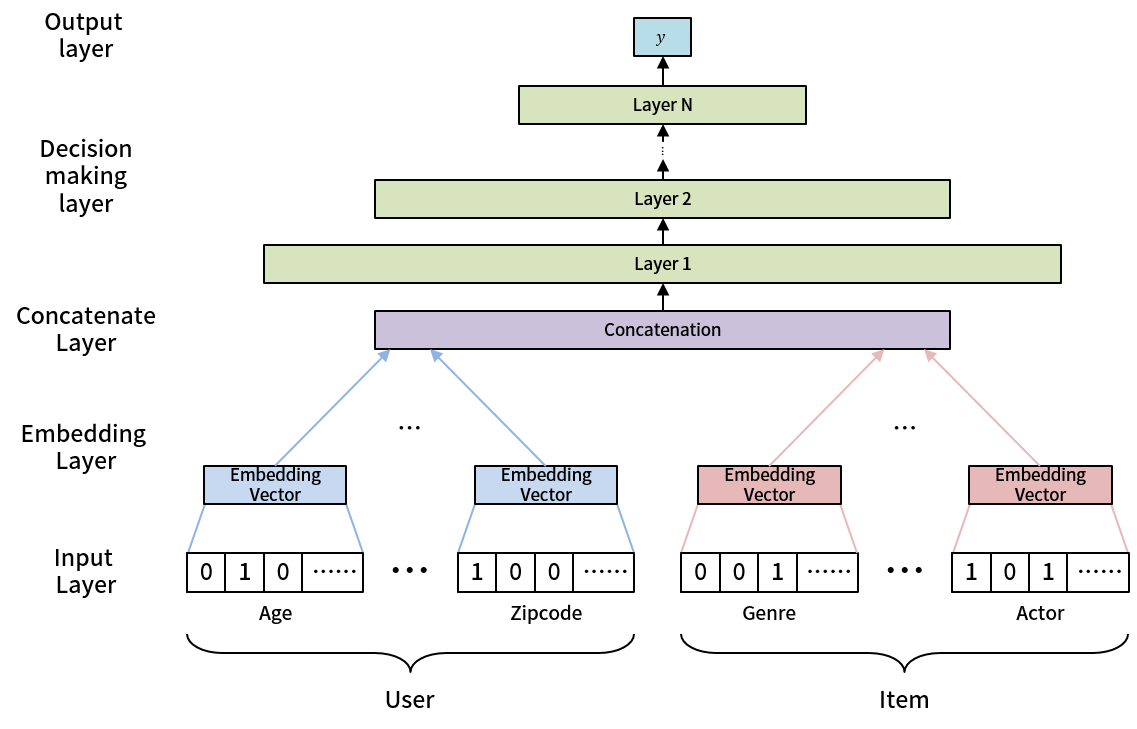
\includegraphics[width=0.7\textwidth]{image/MeLU-arch.png} 
    \caption{MeLU's User preference estimatior.}
    \label{fig:melu-estimator} 
\end{figure}

\begin{figure}[H] 
    \centering 
    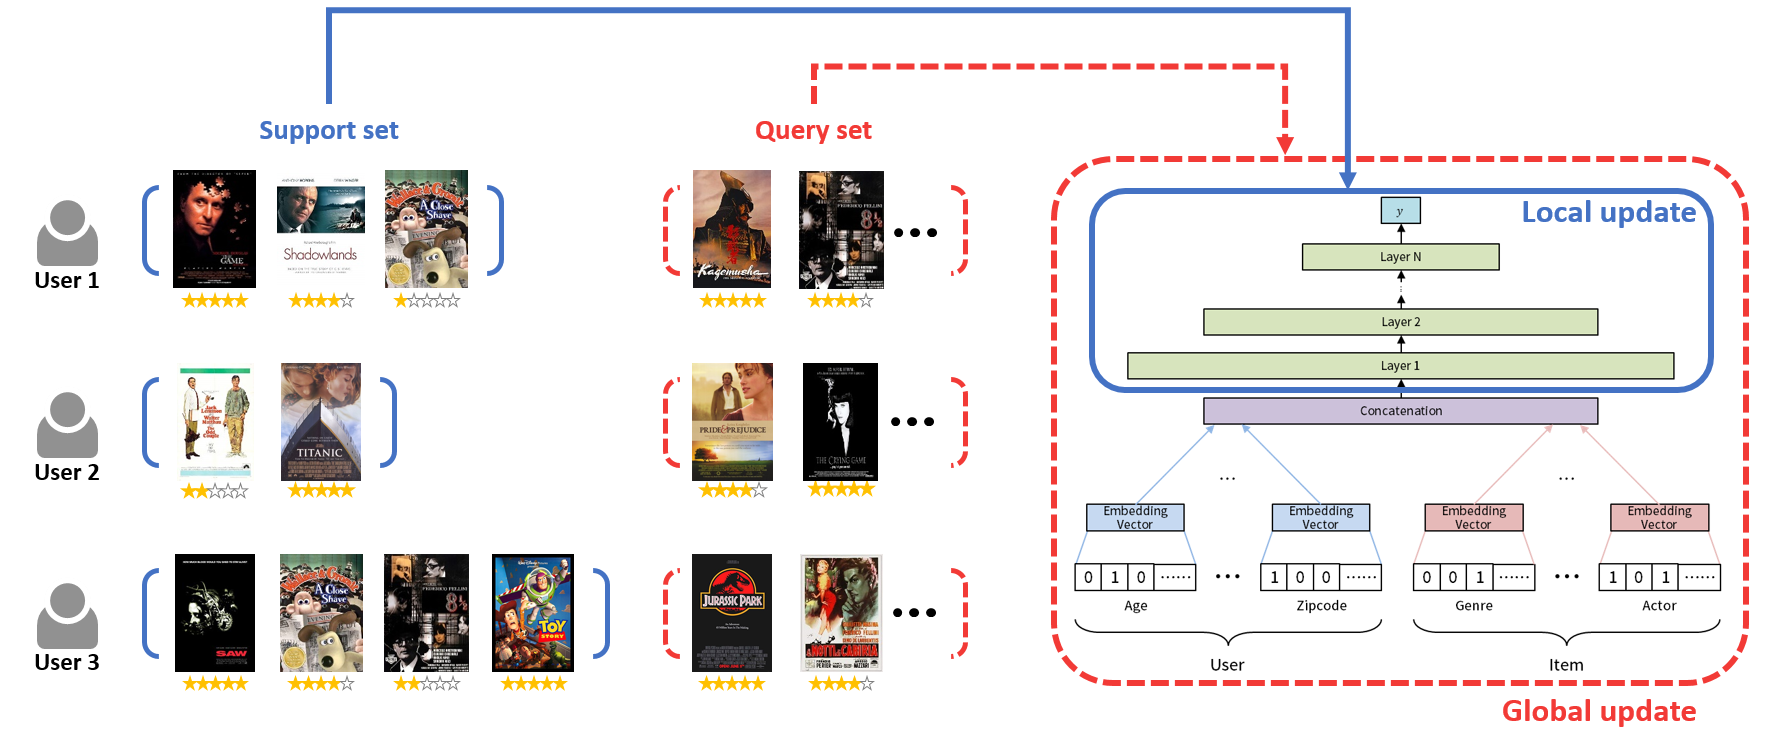
\includegraphics[width=0.7\textwidth]{image/MeLU-update.png} 
    \caption{MeLU's User preference estimatior.}
    \label{fig:melu-updates} 
\end{figure}


\subsection{MeLU's Method}
For user recommendation, MeLU first introduce a user preference estimator\ref{fig:melu-estimator} that consists of decision-making layers and output layer with user and item embeddings. MeLU model takes as input users' information and items' information, together generate an concatenated layer, and then put the concatenation into neural networks as decision making layer, and finally output a result, estimating user's preference for the item. 

Taking the standard MAML approach to meta-learn how to adapt swiftly, the model locally updates the parameters for user i in the batch by backpropagating the following loss function. 
$\mathcal{L}_i = \frac{1}{\left | H_i \right | } \sum_{j\in H_i} (y_{ij} - \hat{y}_{ij})^2 $

For the local update, each local models will update the decision making layers and output layer based on user's unique item-consumption history. While for the global update, the meta-object, it will update both the decision making layers and output layer and embedding vectors of embedding layers, which means that our model assumes users and items do not change, only the users’ thoughts change as they interact with the items. The main different here between classic MAML and MeLU is that MeLU have assumptions for the model and update metrics, due to the specific workload characteristics. The relationship between global and local updates is illustrated in figure\ref{fig:melu-updates}. Furthermore, to improve the model performance in this scenario, MeLU do not limit the length of the item-consumption history and extend the idea of one of the most famous meta-learning algorithms, the matching network. After this optimization, the model shows good performance even when the length of the support set is not fixed across tasks.

The algorithm of MeLU is described in detail in algorithm\ref{algo-melu}.

\begin{algorithm}
    \caption{MAML for User Preference Estimator}
    \label{algo-melu}
    \begin{algorithmic}[1]
        \REQUIRE $\alpha, \beta$: step size hyperparameters
        \STATE randomly initialize $\theta_1$ (embedding vectors for the user and items)
        \STATE randomly initialize $\theta_2$ (weight matrix and bias vector for the decision-making layers)
        \WHILE {not converged}
        \STATE Sample batch of users $B \sim p(\mathcal{B})$
        \FOR {user i in B}
        \STATE set $\theta_2^i$ = $\theta_2$ 
        \STATE Evaluate $\nabla_{\theta_2^i} \mathcal{L}_i (f_{\theta_1,\theta_2^i})$
        \STATE local update $\theta_2^i \longleftarrow  \theta_2^i - \alpha\nabla_{\theta_2^i} \mathcal{L}'_i (f_{\theta_1,\theta_2^i})$
        \ENDFOR
        \STATE global update $\theta_1 \longleftarrow \theta_1 - \beta \sum_{i\in B}\nabla_{\theta_1} \mathcal{L}'_i (f_{\theta_1,\theta_2^i}) $   \\
        $\theta_2 \longleftarrow \theta_2 - \beta \sum_{i\in B}\nabla_{\theta_2} \mathcal{L}'_i (f_{\theta_1,\theta_2^i}) $  
        \ENDWHILE
    \end{algorithmic}
\end{algorithm}

MeLU also provide candidate selection strategy, that select typical evidence candidate which can help the model learn faster about users' preference for different products. 
This strategy can quickly analyze the distinguishing items of the personal preferences of new users in the system. In the model of this article, the larger the average Frobenius norm of the entire user's personalized gradient, the better the difference between user preferences. When calculating the gradient, we modify |·| to indicate the absolute value of the input to backpropagate the unit error. Although products with large gradients can be used to identify user preferences, it may be difficult to make appropriate evaluations when users do not understand the product. Therefore, we also consider the user’s understanding of the product. We assume that the more frequently the user interacts with the product, the better the user understands the product. Therefore, for each item, we use the existing full user-item pairs to calculate the gradient-based value and the popularity-based value as the average Frobenius norm and the number of interactions for each product. In order to scale the unit of two values, we normalize the value to a range from zero to one, and then assign a score to each item by multiplying the two normalized values. Finally, we define the top k items with the highest scores as commodity candidates.

The collaboration between this modified MAML algorithm, specifically for recommendation scenario, and the evidence candidate selection strategy , solve the few-shot learning problem in cold-start recommendation systems better than other similar ML/DL systems. 
\section{Conclusion}

This paper describe a novel algorithm MAML, Model-Agnostic Meta Learning, offers a general approach to adapt meta-learning for most ML algorithms based on gradient descent. 
This methods has a lot of benefits. Firstly, it a simple and easy to understand approach to take, because it doesn't introduce any learned parameters for meta-learning. So that it can be combined with any model representation that is amenable to gradient-based training. Our case study shows that MAML can be applied to few-shot supervised learning problems like classification, regression, as well as few-shot reinforcement learn tasks. What's more, MAML is typically meta-learning the initial parameter (or a weight initialization), adaptation can be performed no matter what amount of data and what number of gradient steps. Simply applying MAML to few-shot image classification problems can already achieve state-of-the-art performance, when the original paper was published. 

\textbf{Future Work} 
Reusing knowledge from past tasks may be a crucial ingredient in making high-capacity scalable models, such as deep neural networks. 
Meta-learning is a huge field while MAML only solved the few-shot learning problems by meta-learning the initial parameters. Other metrics including robustness of ML can also be meta-learned for other cases, while other meta-learning approach like  metric-based,model-based can also be taken. With the thriving of ML academic research, learning techniques and concepts like long short-term memory, attention, neural networks, architecture search also bring opportunities to new meta-learning algorithms.
With opportunities also comes open problems. For example, diverse and multi-modal task distributions.Many big successes of meta-learning have been within narrow task families, while learning on diverse task distributions can challenge existing methods. How to learn more general knowledge just like human beings remain an interesting while challenging open problem for both computer scientists, neural scientists, philosopher and anthropologist. Let's hope meta-learning can bring mankind new understanding of themselves and their existence .




\bibliographystyle{plain}
\bibliography{reference}

\end{document}

% \section{Problem description}
% So far, we have an algorithm $A$ which estimates in correct range of $\eps$ with probability $\ge 0.9$. Our new algorithm $A^{\ast}$ will output in range of $\eps$ with probability $1-\delta$.
% Algorithm:
% \begin{itemize}
% \item Repeat $A$ for $m=O(log (1/\delta))$ times
% \item Take median of all the $m$ answers.
% \end{itemize}

% To prove the correctness, we'll use Chernoff/Hoeffding bounds.

% \begin{definition}
% [Chernoff/Hoeffding Bound]
% Let $X_{1}$, $X_{2}$, $\ldots$, $X_{m}$ be independent random variables $\in \{0,1\}$,
% $\mu = E[\Sigma_{i} X_{i}], \eps \in [0,1]$.
% Then $Pr[|\Sigma_{i} X_{i}-\mu| > \eps\mu] \leq 2e^{-\eps^{2}\mu/3}$
% \end{definition}

% Define $X_{i} = 1$ iff the $i^{th}$ answer of $A$ is correct (i.e. estimated value of $A$ lies in correct range).

% \begin{claim}
% $E[X_{i}] = 0.9$, and $E[\mu] = 0.9m$
% \end{claim}

% \begin{proof}
% Since A is correct with probability 0.9, $E[X_{i}] = 0.9$. And $E[\mu] = 0.9m$ due to linearity of expectation.
% \end{proof}

% \begin{claim}
% New algorithm $A^{\ast}$ is correct when $\Sigma_{i} X_{i} > 0.5m$
% \end{claim}

% \begin{proof}
% Since we are considering median value to be our answer, if more than half the trials of A are correct, algorithm $A^{\ast}$ is also correct.
% \end{proof}

% \begin{claim}
% To prove, $Pr[\Sigma_{i} X_{i} \ge 0.5m] \ge 1-\delta$ or $Pr[\Sigma_{i} X_{i} < 0.5m] < \delta$
% \end{claim}

% \begin{proof}
% \begin{equation}
% \begin{split}
% Pr[\Sigma_{i} X_{i} < 0.5m] & = Pr[\Sigma_{i} X_{i} - 0.9m < -0.4m]\\
% & \le Pr[|\Sigma_{i} X_{i} - \mu| > 0.4m]\\
% & = Pr[|\Sigma X_{i} - \mu| > 0.4/0.9 \mu]
% \end{split}
% \end{equation}
% Using Chernoff bound,
% \begin{equation}
% \begin{split}
% & \leq e^{-c*0.9m}\\
% & < \delta
% \end{split}
% \end{equation}
% Above equation holds for $m = O(log(1/\delta))$
% \end{proof}

% \section{Distinct Elements}
% Given, a stream of size $m$ containing numbers from $[n]$, we have to approximate the number of elements with non-zero frequency. To calculate the exact value the space required:

% \begin{itemize}
% \item $O(n)$ bits. (maintain a vector of length n).
% \item $O(m \log (n))$ bits. (save m numbers, each taking $log(n)$ bits).
% \end{itemize}

% Since, this complexity is not feasible as $m$,$n$ can be very large, we'll look at algorithm for approximating the distinct count value.

% \subsubsection{Hash Function}
% \begin{itemize}
% \item $h : [n] \rightarrow [0,1]$
% \item $h(i)$ is uniformly distributed in $[0,1]$.
% \end{itemize}

% \subsection{Algorithm [Flajolet-Martin 1985]}
% We maintain a variable $z$.
% \begin{enumerate}
% \item Initialize $z = 1$.
% \item Whenever $i$ is encountered: $z = \min{(z,h(i))}$
% \item When done, output $1/z -1$.
% \end{enumerate}

% Now, we'll prove the algorithm works in a similar fashion followed in previous lecture.
% Let $d$ be number of distinct elements.

% \begin{claim}
% $E[z] = d+1$
% \end{claim}

% \begin{proof}
% $z$ is the minimum of $d$ random numbers in $[0,1]$. Pick another random number $a \in [0,1]$. The probability $a<z$:
% \begin{enumerate}
% \item exactly z
% \item probability it's smallest among $d+1$ reals : $1/(d+1)$
% \end{enumerate}
% Equating these two, one can prove the claim.
% \end{proof}

% \begin{claim}
% $\text{var}[z] \leq 2/d^{2}$
% \end{claim}

% \begin{proof}
% It can be done in a similar fashion described in previous lecture.
% \end{proof}

% \subsubsection{$(1+\eps)$ approximation Algorithm }
% We can take $Z = (z_{1} + z_{2} + ... z_{k})/k$ for independent $z_{1}, ... z_{k}$

% \subsection{Alternate Algorithm: Bottom-k}
% Instead of just use the minimum value of hash function for $i$ inputs, we'll maintain the $k$ smallest hashes seen.
% \begin{enumerate}
% \item Initialize $(z_{1}, z_{2},...z_{k}) = 1$.
% \item Keep $k$ smallest hashes seen, s.t. $z_{1}\leq z_{2}\leq...z_{k}$
% \item When done, output $\hat{d} = k/z_{k}$
% \end{enumerate}

% \begin{claim}
% The following claims are stated:
% \begin{itemize}
% \item $Pr[\hat{d} > (1 + \eps)d] \leq 0.05$
% \item $Pr[\hat{d} < (1 - \eps)d] \leq 0.05$
% \item Overall probability that $\hat{d}$ outside range is at most 0.1
% \end{itemize}
% \end{claim}

% \begin{proof}
% To compute $Pr[\hat{d} > (1+\eps)d]$:
% \begin{itemize}
% \item Define $X_{i} = 1$ iff $h(i) < \dfrac{k}{(1+\eps)d}$
% \item Then $\hat{d} > (1+\eps)d$ iff $\Sigma_{i} X_{i} > k$
% \item if $\Sigma_{i} X_{i} > k$\\
%   $\iff \exists$ at least $k$ numbers for which $h(i) < \dfrac{k}{(1+\eps)d}$\\
%     \begin{equation}
%       \iff z_{k} < \dfrac{k}{(1+\eps)d}
%       \iff \dfrac{k}{z_{k}} > (1+\eps)d
%       \iff \hat{d} > (1+\eps)d
%     \end{equation}
% \item
%   $E[X_{i}] = \dfrac{k}{(1+\eps)d}$\\
%   $E[\Sigma_{i} X_{i}] = d E[X_{i}] = \dfrac{k}{1 + \eps}$\\
%   $\text{var}[\Sigma_{i} X_{i}] = d \text{var}[X_{i}] \leq dE[X_{1}^{2}] \leq  \dfrac{k}{1+\eps} \leq k$\\
%   (Since $X_{1} \in \{0,1\}$, $E[X_{1}^{2}] = E[X_{i}]$)
% \item By Chebyshev:
%     $Pr[|\Sigma X_{i} - \dfrac{k}{1+\eps}| > \sqrt{20k}] \leq 0.05 \implies Pr[\Sigma X_{i} > \dfrac{k}{1+\eps} + \sqrt{20k}] \leq 0.05 $\\
%     \begin{itemize}
%     \item
%       (For $\eps < 1/2$ and $k=c/\eps^{2}$)\\
%       $\dfrac{k}{1+\eps} + \sqrt{20k} \leq k(1-\eps+\eps^{2}) + \sqrt{20k}$ (Taylor Series Expansion)\\
%       $ \leq k - k\eps/2 + 5\sqrt{c}/\eps$
%       $ = k - c / 2\eps + 5\sqrt{c}/\eps$\\
%       $ < k $ where $c > 100$
%     \item
%       Since $k > \dfrac{k}{1+\eps} + \sqrt{20k} $ in our case and $\Sigma X_{i}$ is monotonically increasing, $Pr[\Sigma X_{i} > k] \leq Pr[\Sigma X_{i} > \dfrac{k}{1+\eps} + \sqrt{20k}] \leq 0.05$

%     \end{itemize}
% \end{itemize}
% \end{proof}

% \subsection{Hash functions in stream}
% The hash function we used has two practical issues: (1) the return value should be a real number. (2) how do we store it?

% Discretization can solve the first issue. Instead of all the real numbers in $[0, 1]$, we use hash function with range $\{0, \frac{1}{M}, \frac{2}{M}, \frac{3}{M}, \ldots, 1\}$. For large $M \gg n^{3}$, the probability that $d \le n$ random numbers collide is at most $\frac{1}{n}$.

% For the second issue, we use pairwise independent function instead of independent function.

% \begin{definition}
% $h: [n] \rightarrow \{1, 2, \ldots M\}$ is pairwise independent if for all $i \ne j$ and $a, b \in [M]$, $\text{Pr}[h(i)=a \land h(j)=b]=\frac{1}{M^2}$
% \end{definition}

% It works because in previous calculation, we only care about pairs. We defined $X_i=1$ iff $h(i)$ is small than a threshold, then we computed $\text{var}[\Sigma X_i] = E[(\Sigma X_i)^2] - E[(\Sigma X_i)^2] = E[X_1X_1 + X_1X_2 + \ldots]- E[(\Sigma X_i)^2]$. Notice that $E[X_iX_j]$ is the same for fully random $h$ and pairwise independent $h$.

% \begin{example}
% [Construct a pairwise independent hash]
% Assume $M$ is a prime number (if not, we can always pick a larger $M$ that is a prime number). We pick $p, q \in \{0, 1, 2, \ldots M-1 \}$ and the hash function $h(i) = pi+q \mod M$. In this construction we only need $O(\log M) = O(\log n)$ space (to store $p, q, M$).
% \end{example}

% \begin{proof}
% $h(i)=a, h(j)=b$ is equivalent to $pi+q \equiv a, pj+q \equiv b$. So $p(i-j) \equiv a-b$ and $p \equiv (a-b)(i-j)^{-1}, q \equiv a - pi$. Since $M$ is a prime number, the unique inverse implies that there is only one pair $(p, q)$ satisfies it. And the probability that pair is chosen is exactly $\frac{1}{M^2}$.
% \end{proof}

% \section{Impossibility Results}

% We have used both approximation and randomization to solve the distinct counting problem with space much less than $\min{(m, n)}$. Now we are wondering: can we omit either approximation or randomization to achieve the same space efficiency? The answer is no.

% \subsection{Deterministic Exact Won't Work}

% First, we will show that there is no deterministic (no randomization) and exact (no approximation) way to solve it.

% Suppose there do exists a deterministic and exact algorithm $A$ and an estimator function $R$ that use space $s \ll n, m$. That is, for a given integer stream, we first run the algorithm $A$ on the stream. As the stream goes $A$ will return middle memory steps, and we obtain the final memory state $\sigma$ after the stream ends. Then we apply $R$ on $\sigma$ to obtain our estimator $\hat{d}$. Since both $A$ and $R$ are deterministic and exact, $\hat{d}$ must equals to the distinct count for the stream.

% We now build a binary representation $x$ of the stream with the following rules: (1) $x \in \{0, 1\}^{n}$, (2) $i$ in stream iff $x_i = 1$. For example, if 1, 3, 5, 6, 7 are in the stream and 2, 4 are not, $x$ will start with 1, 0, 1, 0, 1, 1, 1. Notice that each stream has a corresponding representation and streams containing different numbers have different representations.

% \begin{claim}
% We can recover the $x$ of the stream given the memory state $\sigma$
% \end{claim}

% \begin{proof}
% Denote $d=R(\sigma)$ be the original estimator. Now we treat $\sigma$ as a middle snapshot of the memory and add integer $i$ as the next element of the stream. Now $A$ will return another memory state $\sigma'$, and $d'=R(\sigma)'$ will be our new estimator. If $d'=d$, $i$ must have appeared in the stream before since $A$ and $R$ are deterministic and exact. Similarly, if $d'>d$, $i$ must have not appeared in the stream before. Using this method with $i=1, 2, 3\ldots$ and we can recover the $x$.
% \end{proof}

% Since we can recover $x$ from $\sigma$, we can treat $\sigma$ as an encoding of a string $x$ of length $n$. But $\sigma$ has only $s \ll n$ bits! Furthermore, we can treat $A$, the function that produces $\sigma$, as a function with domain $\{0, 1\}^{n}$ and $\{0, 1\}^{s}$. We can see that $A$ must be injective because if $A(x)=A(x')=\sigma$, the recoverability implies $x=x'$.

% Hence $s \ge n$. Which implies that there is no deterministic and exact algorithm $A$ and an estimator function $R$ that use space $s \ll n, m$.

% \subsection{Deterministic Approx. Won't Either}

% We can use the similar strategy to prove that deterministic approx. won't work. We pick $T \subset \{0, 1\}^{n}$ that satisfies the following conditions: (1) for all distinct $x, y \in T$, the number of digits $i$ that $y_i=1$ and $x_i=0$ should $\ge \frac{n}{6}$. (2) $|T| \ge 2^{\Omega(n)}$. Now we use algorithm $A$ to encode an input $x$ into $\sigma=A(x)$ and our estimator would be $\hat{d}=R(\sigma)$.

% Now we want to recover $x$ based on $\sigma$, as what we have done in the last section. For a given $\sigma$ and any $y \in T$, we append $y$ to the stream and apply $A$ on it, and $A$ will return a memory state $\sigma'$. Using $\sigma'$ we have new estimator $\hat{d'}=R(\sigma')$.

% \begin{claim}
% If $\hat{d'} > 1.01 \hat{d}$, then $x \ne y$, else $x=y$.
% \end{claim}

% \begin{proof}
% The idea is that when $x=y$, $\hat{d}$ would be really close to $\hat{d'}$ (up to $(1+\epsilon)^{2}$ because both of them are $\epsilon$-approximated) and when $x \ne y$, the construction of $T$ guarantee that $\hat{d} \ge \hat{d} + \frac{n}{6}$. So we can pick an $\epsilon$ that works for our claim.
% \end{proof}

% We can use this method to check every element $y \in T$ to see if $y=x$, and eventually we can recover $x$ from it. Similar to last section, we can show that $A$ is an injective function and it implies that $2^{s} \ge |T|$ or $s = \Omega(n)$.

% \section{Concluding Remarks}

% \begin{itemize}

%   \item We can use median trick and Chernoff bound to improve the probability of an existing algorithm.

%   \item For distinct elements problem, we can also store the hashes $h(i)$ approximately. One example is to store the number of leading zeros, and it only cost $O(\log \log n)$ bits per hash value, and that is the idea behind another algorithm called HyperLogLog.

%   \item For the impossibility results, we can also prove that randomized exact algorithm won't work.

% \end{itemize}